%------------------------------------------------------------------------------
% Manual do HuugleEngine
%------------------------------------------------------------------------------


%------------------------------------------------------------------------------
% Modelo book de documento. Configurado para papel a4 e fonte de 12 pontos. A
% opção openany evita que seja gerada uma página em branco logo após o índice.
%------------------------------------------------------------------------------
\documentclass[a4paper,12pt,openany]{book}
%------------------------------------------------------------------------------
%  Utiliza idioma Português do Brasil e codificação utf8 para exibir caracteres
%  acentuados.
%------------------------------------------------------------------------------
\usepackage[brazilian]{babel}
\usepackage[utf8]{inputenc}
%------------------------------------------------------------------------------
% Pacotes que acrescentam mais recursos ao texto com notação matemática
%------------------------------------------------------------------------------
\usepackage{amsmath,amsfonts,amssymb}
%------------------------------------------------------------------------------
%  Pacote gráfico para incluir figuras no documento.
%------------------------------------------------------------------------------
\usepackage{graphicx}
%-----------------------------------------------------------------------------
% Pacote para criar minipages de fundo colorido e manipulação de cores em
% geral.
%-----------------------------------------------------------------------------
\usepackage[svgnames]{xcolor} 
%-----------------------------------------------------------------------------
% Define cores de fundo para minipages, layout de código fonte java, etc...
%-----------------------------------------------------------------------------
\definecolor{lightblue}{RGB}{173,216,230} 
\definecolor{lightgrey}{RGB}{211,211,211}
\definecolor{greyforcomments}{RGB}{170,170,170}
\definecolor{orange}{RGB}{255,165,0}
%-----------------------------------------------------------------------------
% Define as margens do documento.
%-----------------------------------------------------------------------------
\usepackage{geometry}
\geometry{left=1cm,right=1cm,top=5cm,bottom=2cm}
%-----------------------------------------------------------------------------
% Configura layout para mostrar códigos Java. OBS: Não vai aceitar caracteres
% acentuados nas linhas de comentários dos códigos Java.
%----------------------------------------------------------------------------
\usepackage{listings}
\lstset{
	language=Java,
	basicstyle=\ttfamily\small, 
	keywordstyle=\color{blue}\bfseries,
	stringstyle=\color{orange},
	commentstyle=\color{greyforcomments},
	morecomment=[s][\color{greyforcomments}]{/**}{*/},
	extendedchars=true, 
	showspaces=false, 
	showstringspaces=false, 
	numbers=left,
	numberstyle=\tiny,
	breaklines=true, 
	backgroundcolor=\color{cyan!10}, 
	breakautoindent=true, 
	captionpos=b,
	xleftmargin=0pt,
	tabsize=4
}

%------------------------------------------------------------------------------
% CONVENÇÕES PARA O TEXTO
%
% Variáveis e nomes de métodos são escritos em itálico
%
% Palavras reservadas do Java e classes são escritas em negrito.
%
%------------------------------------------------------------------------------
\begin{document}



\begin{figure}[h]
	
	\centering % para centralizarmos a figura
	
\includegraphics[width=15cm]{Figuras/h.png} 
\end{figure}

\author{Versão 1.1}
\title{Huugle - Manual de Uso}
\date{\today}

\maketitle

%------------------------------------------------------------------------------
%  Cria um índice do documento nomeado como Índice
%------------------------------------------------------------------------------
\renewcommand{\contentsname}{Índice}
\tableofcontents

\newpage

%------------------------------------------------------------------------------
% Neste capítulo introdutório da documentação devem ser definidos os objetivos
% do projeto. E fornecidas quaisquer informações gerais necessárias para a 
% melhor compreensão do projeto.
% 
% Devem ser documentados aqui também o relacionamento deste projeto com outros 
% projetos da biblioteca que porventura estejam sendo utilizados. Por exemplo:
% se o projetoA usa classes de um projetoB, esta informação deve ser documentada
% aqui, explicando-se a função que as classes do projetoB desempenham neste
% projetoA.
%------------------------------------------------------------------------------
\chapter*{Simples Ferramenta de Pesquisa}
\addcontentsline{toc}{chapter}{Simples Ferramenta de Pesquisa}


\paragraph{Entre 18 de janeiro de 2005 e 1 o de fevereiro de 2020 milhares de usuários puderam participar do Fórum
Clube Cético. Para muitos esse período, ou parte dele, representou uma rica experiência de aprendizado
e crescimento pessoal.}
\paragraph{Huugle é um simples aplicativo desenvolvido em Java para ajudar a localizar tópicos e postagens de
interesse no acervo do antigo fórum, atualmente desativado.}




\newpage

%*****************************************************************************
% As próximas seções "part" documentam, cada uma, um dos pacotes que constituem
% o projeto.
%*****************************************************************************
 
%------------------------------------------------------------------------------
% Cada seção "part" deste documento deve ser referente a um pacote do projeto.
%
% O texto no início de cada seção "part" aborda e elucida a função do pacote no
% projeto a que ele pertence.
%------------------------------------------------------------------------------
\colorbox{lightblue}
{
	
\begin{minipage}{18cm}
	
\part*{Histórico do Projeto}
\addcontentsline{toc}{part}{Histórico do Projeto}


\paragraph{Um breve histórico -}
Alguns dias antes do CC sair definitivamente do ar, um grupo de foristas
já havia salvo todas as páginas e arquivos necessários para reconstruir uma imagem estática que fosse um simulacro razoavelmente realista do Clube Cético. Com o objetivo de não só preservar a memória e o conhecimento ali acumulado, como também proporcionar uma experiência de navegação pelo acervo que se aproximasse daquela que os usuários do fórum já estavam acostumados.

\paragraph{}
O resultado foi considerado bastante satisfatório, permitindo que qualquer um instale a cópia reconstruída em seu próprio desktop e utilize um navegador para acessar o material baixado quase da mesma forma como faria se o CC ainda estivesse online.

\paragraph{}
No entanto logo ficou claro que faltava algo fundamental para um material destinado a ser fonte de referência e consulta: uma ferramenta que ajudasse a encontrar o que se buscava em um acervo tão vasto como este que foi compilado. Compreendendo cerca de 1 milhão de postagens distruibuídas por 25010 tópicos publicados ao longo de mais de 15 anos de existência do fórum.

\paragraph{}
Dessa constatação surgiu o projeto do Huugle.

\paragraph{}
Um aplicativo que não tem a pretensão de se equiparar às ferramentas de busca populares com as quais estamos habituados, mas se esforça para ser um mero quebra-galho em alguma medida útil à finalidade bastante específica a que se destina.\\\\\\\\\\\\\\\\\\\\\\\\\\\\\\\\


\end{minipage}


}%fim da caixa de texto com fundo colorido

\newpage

%*****************************************************************************
% As próximas seções "chapter" documentam, cada uma, uma das classes que
% constituem o pacote documentado nesta seção "part".
%*****************************************************************************

%------------------------------------------------------------------------------
% Documenta a primeira classe do pacote. 
%------------------------------------------------------------------------------
\colorbox{lightgrey}{
	
\begin{minipage}{18cm}
	
\chapter*{Utilização}
\addcontentsline{toc}{chapter}{Utilização}

\paragraph{Como procurar tópicos e postagens -}
Huugle possui uma única janela principal onde é possível digitar os termos a serem pesquisados, assim como definir parâmetros que restringem o escopo da pesquisa.

\paragraph{}
No centro dessa janela há um painel onde é possível inserir até 6 termos e o programa, em seu modo default, irá retornar uma lista contendo todos os tópicos que apresentam pelo menos uma destas palavras em seu título. O que pode ser alterado para realização também de pesquisas em postagens de foristas.

\paragraph{}
A um clique no botão Pesquisar, uma janela exibe o progresso do processo de pesquisa, findo o qual deverá ser aberta uma aba no navegador padrão com uma lista de links para os resultados encontrados.



\end{minipage}



}%fim da caixa de texto com fundo colorido

\begin{figure}[h]
	\caption{Janela Principal}
	
	\centering % para centralizarmos a figura
	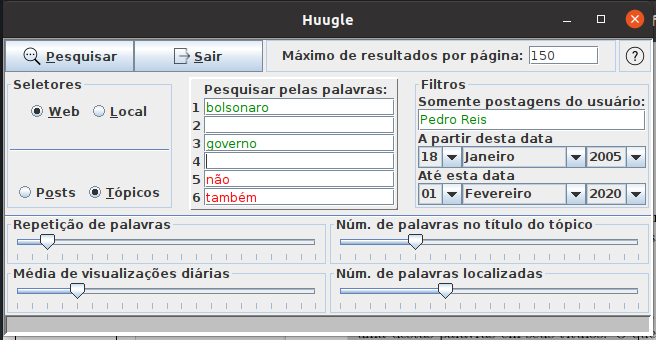
\includegraphics[width=15cm]{Figuras/janela-principal.png} % leia abaixo
	\label{figura:qualquernome}
\end{figure}

\newpage

%*****************************************************************************
% As próximas seções "section" documentam, cada uma, um dos métodos que
% constituem a classe documetada  nesta seção "chapter".
%*****************************************************************************

%------------------------------------------------------------------------------
% Documenta primeiro método da classe a qual é referente esta seção "chapter".
%------------------------------------------------------------------------------
\section*{Usando filtros}
\addcontentsline{toc}{section}{Usando filtros}

\paragraph{}
Os resultados podem ser filtrados, fazendo com que apenas postagens ou tópicos publicados por um determinado autor sejam retornados como resultados da busca. Porém se não existia um forista regsitrado com o \textit{nick} que foi digitado no campo de entrada, este mesmo campo indicará exibindo-o com cor vermelha. Nesse caso a busca pelos termos pesquisados se dará para \textit{posts} ou títulos de tópicos de qualquer forista. Da mesma que forma que seria se este campo fosse deixado em branco.

\begin{figure}[h]
	\caption{Usando Filtros}
	
	\centering % para centralizarmos a figura
	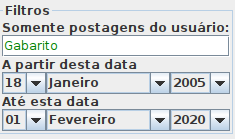
\includegraphics[width=12cm]{Figuras/usando-filtros.png} % leia abaixo
	\label{figura:qualquernome}
\end{figure}

\paragraph{}
Também a pesquisa pode ser restrita a um intervalo entre duas datas.
\paragraph{}
Um intervalo entre 18 de janeiro de 2005 e 1º de fevereiro de 2020 retorna todos os resultados possíveis. Pois esse período corresponde ao tempo de existência do fórum.
\paragraph{}
Configurar uma data inicial posterior à data final necessariamente retornará uma lista de resultados vazia.
[figura 2 - Usando filtros]

\section*{Como especificar os termos a serem pesquisados}
\addcontentsline{toc}{section}{Como especificar os termos a serem pesquisados}

\paragraph{}
No painel no centro da janela principal até 6 palavras chave podem ser inseridas.
\paragraph{}
Estas caixas de texto só aceitam caracteres de palavra e apenas letras minúsculas. Uma busca por abacaxi seria o mesmo que uma busca por Abacaxi ou ABACAXI (ou mesmo AbACaXi). No entanto os acentos fazem diferença e pesquisar por ”pele” não é o mesmo que pesquisar por ”pelé”.

\begin{figure}[h]
	\caption{Pesquisa Padrão}
	
	\centering % para centralizarmos a figura
	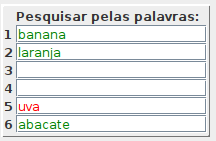
\includegraphics[width=15cm]{Figuras/pesquisa-padrao.png} % leia abaixo
	\label{figura:qualquernome}
\end{figure}

\paragraph{}
Estas caixas de texto rejeitam a digitação de dígitos, pontuação, símbolos especiais, espaço em branco e também letras maiúsculas. O que significa que as teclas para estes caracteres não irão "funcionar" se você estiver tentando digitar um termo a ser pesquisado em um dos campos de entrada. Apenas letras minúsculas formando palavras simples de 4 a 16 caracteres
 constituem termos válidos para busca. E campos podem ser deixados em branco também.
\paragraph{} 
Não é possível digitar palavras com mais de 16 caracteres, porém é possível digitar uma palavras com menos de 4 caracteres. Nesse caso, ao perder o foco, o campo exibirá o termo em vermelho, uma vez que o Huugle não faz pesquisa para termos com menos de 4 caracteres.
\paragraph{}
Também, para manter os arquivos de índice em um tamanho conveniente, palavras muito comuns como, por exemplo,  "isso" ou "minha", não foram indexadas. Se o usuário tentar buscar por uma palavra não indexada o campo de entrada exibirá o termo digitado em vermelho ao perder o foco.
\paragraph{} 
Termos válidos serão exibidos na cor verde.
\paragraph{}
A lista completa de palavras não indexadas se encontra no arquivo \textbf{excludeds.dat} presente na pasta \textit{database}.
\paragraph{}
Por padrão, o programa faz tanto uma busca \textbf{AND} quando uma busca \textbf{OR} por estes termos. Ou seja, serão retornadas postagens que contenham no texto pelo menos uma destas palavras ou qualquer combinação
destas. O mesmo quando a busca é feita para títulos de tópicos: serão retornados tópicos que contenham em seu título pelo menos uma ou qualquer combinação das palavras digitadas.
\paragraph{}
Isso pode ser alterado de duas formas:
\paragraph{}
- Colocando-se um sinal de mais (+) antes dos termos, força-se a busca a retornar apenas resultados que contenham todas as palavras precedidas por um sinal de mais (+). E o mesmo para buscas em títulos de tópicos: somente títulos com todas as palavras que foram precedidas por (+) serão retornados. Se houver.
\paragraph{}
Nesse caso, quando há pelo menos um termo precedido por (+), nenhum outro termo eventualmente inserido será pesquisado. Uma vez que estas inserções se tornam irrelevantes já que o que irá determinar um resultado válido serão somente os termos precedidos por sinal de mais.
\paragraph{}
- Também precedendo os termos por um sinal de menos (-) podemos alterar a forma como o programa fará a busca. Dessa maneira apenas resultados que \textbf{não} contiverem nenhuma das palavras precedidas por um sinal de menos poderão ser retornados.

\begin{figure}[h]
	\caption{Prefixando com (+) e (-)}
	
	\centering % para centralizarmos a figura
	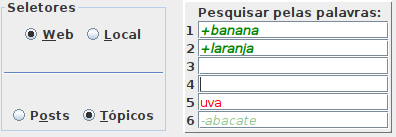
\includegraphics[width=15cm]{Figuras/outra-forma-de-pesquisar.png} % leia abaixo
	\label{figura:qualquernome}
\end{figure}
\paragraph{}
No exemplo da figura 4, todos os tópicos que contivessem "banana"  \textbf{E} "laranja" em seus títulos mas nenhuma ocorrência da palavra ”abacate” seriam retornados como resultados válidos da pesquisa. E apenas estes
seriam resultados válidos. (Note que "uva" não foi incluída na pesquisa por ter menos de 4 caracteres).

\section*{Critérios para determinar relevância de resultados}
\addcontentsline{toc}{section}{Critérios para determinar relevância de resultados}
\paragraph{}
Resultados de uma busca serão listados por ordem de relevância. Com aqueles supostos como mais prováveis de serem os resultados almejados sendo apresentados no topo da lista.
\paragraph{}
O programa considera 4 critérios para determinar a provável relevância de resultados:
\paragraph{}
- O número de vezes que as palavras digitadas ocorrem no texto de uma postagem quando a busca é para textos de postagens ou o números destas ocorrências em títulos de tópicos quando a busca é para tópicos.
\paragraph{}
- Se os termos buscados ocorrem também no título do tópico onde foi publicada a postagem (apenas para buscas em textos de postagens).
\paragraph{}
- A média de visualizações de um tópico. Sendo resultados associados a tópicos mais visualizados considerados mais relevantes.
\begin{figure}[h]
	\caption{Rankeamento dos Resultados Obtidos}
	
	\centering % para centralizarmos a figura
	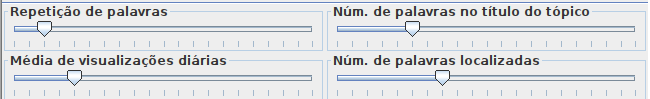
\includegraphics[width=15cm]{Figuras/ajustando-relevancia.png} % leia abaixo
	\label{figura:qualquernome}
\end{figure}
\paragraph{}
- E por fim quantos, dos termos especificados, ocorrem em um resultado. Uma fórmula é utilizada para quantificar todos estes critérios em um único número que representa o
ranking de relevância de um resultado.
\paragraph{}
$2 \cdot w_{1} \cdot FP + 10 \cdot w_{2} \cdot PT + 10 \cdot w_{3} \cdot \log_2 {V} + 100 \cdot w_{4} \cdot (OP - 1)$
\paragraph{}
Onde:
\paragraph{}
FP indica o número de vezes que palavras digitadas ocorrem nos resultados (em títulos de tópicos ou textos de postagens). Se, por exemplo, os termos são ”governo” e ”brasil”em uma pesquisa buscando os termos em textos de postagens e ”governo” ocorreu duas vezes em um determinado \textit{post} onde ”brasil” ocorreu três vezes, então FP = 2 + 3 = 5
\paragraph{}
PT é o número de palavras digitadas que ocorreram também no título do tópico. Assim uma busca por ”governo” e ”brasil” que retornasse como resultado uma postagem do tópico ”Governo Bolsonaro” atribuiria valor 1 a PT. Pois o termo ”governo” também está presente no título do tópico onde foi publicado o \textit{post}.
V é o cálculo da média de visualizações diárias de um tópico. É o número total de visualizações de um tópico dividido pelo número de dias transcorridos desde a publicação do tópico até a data de encerramento do Clube Cético, em 1º de fevereiro de 2020.
\paragraph{}
Para efeito de cálculo, a fórmula utiliza o logaritmo de V na base 2 como um expediente para atenuar a tendência que essa expressão teria de apontar como extremamente relevantes postagens em tópicos que tinham números desproporcionalmente altos de visualizações.
\paragraph{}
Se faz necessário porque os tópicos mais visualizados (com visualizações muito superiores à média) seriam, paradoxalmente, resultados não preferenciais para a maioria das buscas. O que se dá pelo fato de serem tópicos sobre distrações e amenidades, muito visualizados no entanto pouco consultados por não suscitarem discussões de interesse.
\paragraph{}
Como exemplos, pode-se citar o tópico da ”Mulher mais gostosa que já vi...” e suas mais de 3 milhões de visualizações ou o ”Muro de Lamentações” visto também mais de um milhão de vezes.
\paragraph{}
OP é o número de palavras digitadas nos campos de busca que ocorrem no \textit{post} ou no título de um tópico. Repetições de uma mesma palavra não são contadas. Assim, se a busca foi por ”laranja”, ”banana” e ”tangerina” e banana ocorre 3 vezes em um dado post, enquanto laranja duas vezes mas tangerina nenhuma, OP receberia valor 2 para esse \textit{post}. Porque ”laranja” e ”banana” ocorrem, independentemente de quantas vezes possa ocorrer um destes termos.
\paragraph{}
Já as variáveis w1, w2, w3 e w4 são pesos que, dependendo do valor que lhes for atribuído conferem maior ou menor relevância a cada um dos critérios, alterando a forma como a lista de resultados é ordenada.
\paragraph{}
Estes pesos podem ser ajustados na interface do programa a partir de 4 controles deslizantes que permitem variar cada um deles entre 0 e 20.
\paragraph{}
O controle ”Repetição de Palavras” atribui o valor ao peso w1. Se for desejado que esse fator seja muito relevante, o controle deve ser deslocado para a direita. Posiciona-lo em zero na escala, totalmente à esquerda, anula o número de repetições de palavras como critério de cálculo de relevância de um resultado.
\paragraph{}
”Número de palavras no título do tópico” determina o valor de w2. Um valor maior para w2 fará com que a ocorrência de palavras digitadas nos títulos de tópicos seja um critério mais significativo quando o programa ordenar a lista de resultados retornados.
\paragraph{}
"Média de visualizações diárias" está associado a w3. Se você está procurando um \textit{post} específico em uma lista com centenas de resultados retornados, e sabe que este \textit{post} não foi publicado em um tópico muito visualizado, posicionar em zero este controle ajuda a colocar o resultado realmente procurado mais para o topo da lista.
\paragraph{}
”Número de palavras localizadas” determina o valor do peso w4. Um valor alto tende a ordenar a lista usando um critério \textbf{AND} e um valor baixo tende a ordenar a lista de resultados por um critério \textbf{OR}.

\section*{Seleção}
\addcontentsline{toc}{section}{Seleção}

\paragraph{}
Pode-se determinar se a pesquisa será feita em títulos de tópicos, retornado apenas tópicos que satisfizerem os critérios escolhidos, ou serão pesquisados os textos de postagens na busca pelos termos inseridos pelo usuário.

\begin{figure}[h]
	\caption{Seletores}
	
	\centering % para centralizarmos a figura
	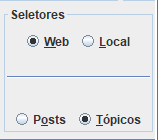
\includegraphics[width=15cm]{Figuras/seletores.png} % leia abaixo
	\label{figura:qualquernome}
\end{figure}

\paragraph{}
Também é possível selecionar se os links na página de resultados apontarão para uma versão online do acervo ou para a cópia local que deve estar instalada em um diretório nomeado clubecetico.org. O mesmo onde deve estar a pasta Huugle contendo o executável desta aplicação.
\paragraph{}
Caso contrário os links para arquivos do acervo local não serão capazes de abrir no navegador as páginas referidas.

\section*{Limitando número de resultados exibidos}
\addcontentsline{toc}{section}{Limitando número de resultados exibidos}

\begin{figure}[h]
	\caption{Limitando Resultados Exibidos}
	
	\centering % para centralizarmos a figura
	
\includegraphics[width=15cm]{Figuras/resultados-por-pagina.png} % leia abaixo
	\label{figura:qualquernome}
\end{figure}

\paragraph{}
Esse campo permite limitar o número de links que será exibido na página do navegador. Se um valor N for inserido neste campo, apenas os N mais relevantes resultados (de acordo com os parâmetros de relevância correntemente configurado) serão mostrados na página.

%-----------------------------------------------------------------------------
% Fim da documetação dos métodos da classe. Pula para próxima página.
%------------------------------------------------------------------------------
\newpage

%------------------------------------------------------------------------------
% A partir dessa tag todos os capítulos são interpertados pelo Latex como 
% apêndices e indexados por letras em vez de números. Serão apêndices da parte
% onde estiverem incluídos. Neste modelo de documento as partes servem para
% documentar pacotes do projeto. Portanto cada documentação de pacote do projeto
% pode ter seus próprios apêndices.
%------------------------------------------------------------------------------
\appendix


\chapter{Aspectos de Engenharia e Limitações da Ferramenta}

\paragraph{}
Huugle realiza a pesquisa sobre uma base de dados que acompanha a distribuição do executável, na forma de arquivos .dat inclusos na pasta \textit{database}. Essa base de dados foi coletada dos arquivos contendo o HTML
bruto de todas as páginas de tópicos e seções do desativado fórum Clube Cético.
\paragraph{}
A referida base de dados possui arquivos indexando palavras catalogadas de textos de postagens, de títulos de tópicos, dados sobre posts, tópicos, usuários, etc...
\paragraph{}
Idealmente, a base de dados deveria associar cada palavra coletada dos textos de postagens, a uma lista contendo os registros de todos posts onde essa dada palavra ocorre. Infelizmente este objetivo se provou impraticável, em face do acervo compreender cerca de um milhão de postagens, o que faria com que o tamanho de alguns arquivos na base de dados dificultasse o download do pacote da aplicação. Uma vez que palavras muito comuns podem ocorrer e ocorrem em até centenas
de milhares de \textit{posts}, o que determinaria que as listas de \textit{posts} associadas a estes termos devessem conter
centenas de milhares de entradas.
\paragraph{}
Por outro lado estes termos muito comuns (palavras como ”também”, ”você”, etc...) não auxiliam muito a refinar uma pesquisa e direcionar a busca à informação que se deseja obter.
\paragraph{}
Consequentemente limitou-se o número de registros que uma palavra pode apontar em cerca de 30.000, o que significa que uma pesquisa em textos de postagens pode não abranger todos os posts onde esta palavra ocorreu, caso seja palavra de uso relativamente comum.
\paragraph{}
O critério utilizado para selecionar ou descartar registros de posts associados a uma dada palavra foi justamente o cálculo do ranking do \textit{post}, já explicado anteriormente neste manual.
\paragraph{}
 Quando a lista de \textit{posts} onde uma dada palavra ocorre alcança seu limite máximo, novos \textit{posts} foram incluídos nesta lista somente em substituição a \textit{posts} já constantes da lista, mas que possuíam ranking menor que o novo registro de \textit{post} candidato à inserção. Ou seja, era sempre o último \textit{post} da lista (o de menor ranking) trocado por algum outro, se o cálculo do ranking deste outro fosse maior que o do último da lista de \textit{posts} já "lotada".
\paragraph{}
Sabendo-se disso, entende-se que uma busca será mais eficiente e terá mais chance de sucesso, se forem utilizados termos pouco comuns. Se alguém procura por um \textit{post} onde sabe que existe a frase ”meu avô tinha alzheimer”, o termo ”alzheimer” tem muito mais chance de conter uma lista com todos os
\textit{posts} onde essa palavra existe, do que ”avô”ou ”tinha”, palavras bem mais comuns.
\paragraph{}
No caso das pesquisas em títulos de tópicos, por se debruçaram em um conjunto de ”apenas” 25010 destes títulos, espera-se que o algoritmo tenha sido capaz de construir uma base de dados completa e portanto
esse tipo de busca não sofre da mesma limitação das pesquisas realizadas em textos de postagens.
\paragraph{}
Porém convém ressaltar que a base de dados não catalogou palavras com menos de 4 caracteres e nem maiores que 16 caracteres. Também não catalogou strings com dígitos, pontuações, símbolos especiais... apenas palavras. E a pesquisa só procura por palavras.


\newpage



\end{document}